%(BEGIN_QUESTION)
% Copyright 2011, Tony R. Kuphaldt, released under the Creative Commons Attribution License (v 1.0)
% This means you may do almost anything with this work of mine, so long as you give me proper credit

Anta at måleren i denne Wheatstone-broen står «i fullt utslag» selv når RTD-en er ved 0$^{o}$ C (når broen egentlig skal være balansert), med polariteten over visningsvoltmeterets terminaler som vist. Du måler 50 millivolt mellom testpunktene {\bf C} og {\bf A} med digitalt multimeter:

$$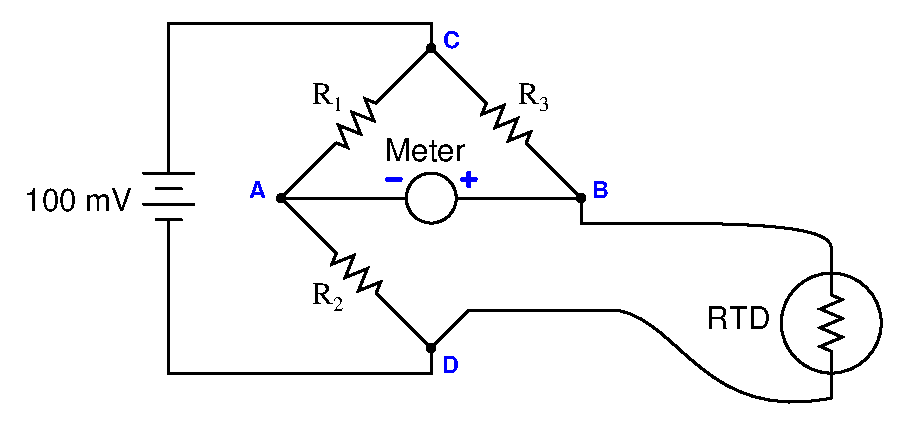
\includegraphics[width=15.5cm]{i00149x01.eps}$$

Vurder sannsynligheten for hver oppgitt feil i kretsen. Vurder én feil av gangen (ingen samtidige feil), og avgjør om hver feil alene kan forklare {\it alle} målinger og symptomer i kretsen.

% No blank lines allowed between lines of an \halign structure!
% I use comments (%) instead, so that TeX doesn't choke.

$$\vbox{\offinterlineskip
\halign{\strut
\vrule \quad\hfil # \ \hfil & 
\vrule \quad\hfil # \ \hfil & 
\vrule \quad\hfil # \ \hfil \vrule \cr
\noalign{\hrule}
%
% First row
{\bf Feil} & {\bf Mulig} & {\bf Umulig} \cr
%
\noalign{\hrule}
%
% Another row
$R_1$ avbrudd &  &  \cr
%
\noalign{\hrule}
%
% Another row
$R_2$ avbrudd &  &  \cr
%
\noalign{\hrule}
%
% Another row
$R_3$ avbrudd &  &  \cr
%
\noalign{\hrule}
%
% Another row
RTD avbrudd &  &  \cr
%
\noalign{\hrule}
%
% Another row
$R_1$ kortsluttet &  &  \cr
%
\noalign{\hrule}
%
% Another row
$R_2$ kortsluttet &  &  \cr
%
\noalign{\hrule}
%
% Another row
$R_3$ kortsluttet &  &  \cr
%
\noalign{\hrule}
%
% Another row
RTD kortsluttet &  &  \cr
%
\noalign{\hrule}
} % End of \halign 
}$$ % End of \vbox

\underbar{file i00149}
%(END_QUESTION)





%(BEGIN_ANSWER)

% No blank lines allowed between lines of an \halign structure!
% I use comments (%) instead, so that TeX doesn't choke.

$$\vbox{\offinterlineskip
\halign{\strut
\vrule \quad\hfil # \ \hfil & 
\vrule \quad\hfil # \ \hfil & 
\vrule \quad\hfil # \ \hfil \vrule \cr
\noalign{\hrule}
%
% First row
{\bf Feil} & {\bf Mulig} & {\bf Umulig} \cr
%
\noalign{\hrule}
%
% Another row
$R_1$ avbrudd &  & $\surd$ \cr
%
\noalign{\hrule}
%
% Another row
$R_2$ avbrudd &  & $\surd$ \cr
%
\noalign{\hrule}
%
% Another row
$R_3$ avbrudd &  & $\surd$ \cr
%
\noalign{\hrule}
%
% Another row
RTD avbrudd & $\surd$ &  \cr
%
\noalign{\hrule}
%
% Another row
$R_1$ kortsluttet &  & $\surd$ \cr
%
\noalign{\hrule}
%
% Another row
$R_2$ kortsluttet &  & $\surd$ \cr
%
\noalign{\hrule}
%
% Another row
$R_3$ kortsluttet & $\surd$ &  \cr
%
\noalign{\hrule}
%
% Another row
RTD kortsluttet &  & $\surd$ \cr
%
\noalign{\hrule}
} % End of \halign 
}$$ % End of \vbox


%(END_ANSWER)





%(BEGIN_NOTES)

{\bf Dette spørsmålet er ment for eksamen og ikke for arbeidsark!}.

%(END_NOTES)
